\documentclass[12pt]{report} % twoside

    \usepackage[top=2cm, bottom=2cm, left=2cm, right=2cm]{geometry}

    % Français
    \usepackage[utf8]{inputenc}
    \usepackage[T1]{fontenc}
    \usepackage[french]{babel}

    % Mathématiques
    \usepackage{amsmath}
    \usepackage{amssymb}
    \usepackage{mathrsfs}
    \usepackage{stmaryrd}
    \usepackage{mathabx}
    \usepackage{pifont} % x c mark

    % Liste / Figure / Tableau
    \usepackage{enumitem}
    \usepackage{float}
    \usepackage{caption}
    \usepackage{multirow}
    \captionsetup{justification=centering}
    \usepackage{longtable}

    % TikZ
    \usepackage{tikz}

    % Autre
    \newcommand{\hr}{\par\noindent\rule{\textwidth}{0.4pt}}

    % Titlesec & Titletoc
    \usepackage{titlesec}
    \usepackage{titletoc} %[rightlabels]
    \renewcommand{\thechapter}{\Roman{chapter}}
    \renewcommand{\thesubsection}{$\bullet$}
        % Title Spacing
        \titlespacing*{\chapter}{0pt}{-30pt}{18pt}
        \titlespacing*{\section}{6pt}{18pt}{14pt}
        \titlespacing*{\subsection}{12pt}{18pt}{11pt}
        % Title Format
        \titleformat{\chapter}[display]
            {\Large\bfseries}
            {}{0pt}{\thechapter.\ }
            [\vspace{0.4pt}\titlerule]
        \titleformat{name=\chapter,numberless}[display]
            {\Large\bfseries}
            {}{0pt}{}
            [\vspace{0.4pt}\titlerule]
        \titleformat{\section}
            {\large}
            {\bfseries\thesection}{1em}{} % \itshape
        \titleformat{\subsection}
            {\large}
            {\thesubsection}{1em}{}
        % Title Contents
        \titlecontents{chapter}[0em]
            {\addvspace{1em}\bfseries}
            {\thecontentslabel\enspace}
            {}
            {\hfill\contentspage}
            [\vspace{2pt}]
        \titlecontents{section}[2em]
            {}
            {\thecontentslabel\enspace}
            {}
            {\dotfill\contentspage}
            [\vspace{1pt}]
        \titlecontents{figure}[2em]
            {}
            {\thecontentslabel\enspace}
            {}
            {\dotfill\contentspage}
            [\vspace{1pt}]
        \titlecontents{table}[2em]
            {}
            {\thecontentslabel\enspace}
            {}
            {\dotfill\contentspage}
            [\vspace{1pt}]
        \titlecontents{subsection}[4em]
            {}
            {\thecontentslabel\enspace}
            {}
            {\dotfill\contentspage}
            [\vspace{0pt}]

    % Code
    \usepackage{color, colortbl}
    \usepackage{listings}

    \definecolor{background}{rgb}{0.99,0.99,0.99}
    \definecolor{border}{rgb}{0.85,0.85,0.85}

    \definecolor{mOrange}{rgb}{1.00,0.47,0.00}
    \definecolor{mOrange2}{rgb}{1.00,0.65,0.00}
    \definecolor{mGreen}{rgb}{0.25,0.60,0.10}
    \definecolor{mBlue}{rgb}{0.23,0.35,0.70}

    \lstdefinestyle{CStyle}{
        language           = C,
        frame              = lines, % single L lr
        %frameround        = {t}{t}{t}{t},
        framerule          = 1pt,
        framexleftmargin   = 2mm,
        %framexrightmargin = 17pt,
        framexbottommargin = 2mm,
        framextopmargin    = 2mm,
        backgroundcolor    = \color{background},
        rulecolor          = \color{border},
        %
        basicstyle      =\ttfamily\footnotesize,
        keywordstyle    = \color{mOrange},
        keywordstyle    = [2]\color{mOrange2},
        %commentstyle   = \color{red},
        identifierstyle = \color{mBlue},
        stringstyle     = \color{mGreen},
        otherkeywords   = {
            >,<,.,:,-,!,=,+,+,/,|,~,&,* % ; [ ]
        },
        morekeywords   = [2]{
            bool,size_t,FILE,
            uint8_t,uint32_t,
            mpError,mpErrorCode,mpErrorType,
            mpChar,mpString,mpCString,
            mpLine,
            mpTag,mpValue,mpToken,mpFetch,
            mpMemory,mpRegister,mpRegister_,
            mpInstruction,mpToMemory,
            mpVector_mpToken
        },
        %
        breakatwhitespace = false,
        breaklines        = true,
        keepspaces        = true,
        numbers           = left,
        numbersep         = 10pt,
        numberstyle       = \footnotesize\ttfamily\color{gray},
        showspaces        = false,
        showstringspaces  = false,
        showtabs          = false,
        tabsize           = 2,
        %aboveskip         = 2em,
        %xleftmargin      =.25\textwidth,
        %xrightmargin     =.25\textwidth,
    }

    \lstset{literate=
        {á}{{\'a}}1 {é}{{\'e}}1 {í}{{\'i}}1 {ó}{{\'o}}1 {ú}{{\'u}}1
        {Á}{{\'A}}1 {É}{{\'E}}1 {Í}{{\'I}}1 {Ó}{{\'O}}1 {Ú}{{\'U}}1
        {à}{{\`a}}1 {è}{{\`e}}1 {ì}{{\`i}}1 {ò}{{\`o}}1 {ù}{{\`u}}1
        {À}{{\`A}}1 {È}{{\'E}}1 {Ì}{{\`I}}1 {Ò}{{\`O}}1 {Ù}{{\`U}}1
        {ä}{{\"a}}1 {ë}{{\"e}}1 {ï}{{\"i}}1 {ö}{{\"o}}1 {ü}{{\"u}}1
        {Ä}{{\"A}}1 {Ë}{{\"E}}1 {Ï}{{\"I}}1 {Ö}{{\"O}}1 {Ü}{{\"U}}1
        {â}{{\^a}}1 {ê}{{\^e}}1 {î}{{\^i}}1 {ô}{{\^o}}1 {û}{{\^u}}1
        {Â}{{\^A}}1 {Ê}{{\^E}}1 {Î}{{\^I}}1 {Ô}{{\^O}}1 {Û}{{\^U}}1
        {Ã}{{\~A}}1 {ã}{{\~a}}1 {Õ}{{\~O}}1 {õ}{{\~o}}1
        {œ}{{\oe}}1 {Œ}{{\OE}}1 {æ}{{\ae}}1 {Æ}{{\AE}}1 {ß}{{\ss}}1
        {ű}{{\H{u}}}1 {Ű}{{\H{U}}}1 {ő}{{\H{o}}}1 {Ő}{{\H{O}}}1
        {ç}{{\c c}}1 {Ç}{{\c C}}1 {ø}{{\o}}1 {å}{{\r a}}1 {Å}{{\r A}}1
        {€}{{\euro}}1 {£}{{\pounds}}1 {«}{{\guillemotleft}}1
        {»}{{\guillemotright}}1 {ñ}{{\~n}}1 {Ñ}{{\~N}}1 {¿}{{?`}}1
    }

    \lstset{
        escapeinside={(*@}{@*)}, % if you want to add LaTeX within your code
    }

\begin{document}

% ========================================================== %
%     PREMIERE PAGE
% ========================================================== %

\hfill {\large 2021} \\

\vspace{5cm}
\begin{center}
    {\Huge Algorithmique et programmation C} \\
        \vspace{1cm}
    {\huge Projet C - Émulateur MIPS}
\end{center}

\newpage

% ========================================================== %
%     SOMMAIRE
% ========================================================== %

\tableofcontents
%\vspace{3em}
\begingroup
    \let\cleardoublepage\relax  % book
    \let\clearpage\relax        % report
    %\listoffigures
    %\listoftables
\endgroup

\newpage

% ========================================================== %
%     INTRODUCTION
% ========================================================== %
\chapter{Introduction}

\paragraph{}
Fichiers commums à tout le projet : {\tiny (à réécrire)}

% ========================================================== %
%     INTRODUCTION : mpType
% ========================================================== %
\section{mpType}

\paragraph{}
Pour éviter les inclusions circulaires, un fichier d'en-tête {\ttfamily mpType.h} est disponible pour y déclarer la grande majorité des types dont les différents modules auront besoin.

% ========================================================== %
%     INTRODUCTION : mpError
% ========================================================== %
\section{mpError}

\paragraph{}
L'émulateur gère une grande quantité d'erreur, ce module est composé d'une fonction {\ttfamily mpRaise} pour faire remonter les erreurs à l'utilisateur :

%\vspace{5mm}
\begin{lstlisting}[
    style=CStyle,
    numbers=none,
    title={\ttfamily mpError.h}
]
void mpRaise(mpError* error);
\end{lstlisting}

\paragraph{}
{\ttfamily mpError} est une structure composée en partie de : un type, un code, la ligne à afficher où occure l'erreur, etc. Tous ces membres sont utilisables seulement si le champ {\ttfamily success} est à true.

%\vspace{5mm}
\begin{lstlisting}[
    style=CStyle,
    numbers=none,
    title={\ttfamily mpType.h}
]
typedef struct
{
    bool        success;

    mpErrorType type;
    mpErrorCode code;

    mpString    context;
    mpString    line;
    mpChar*     col;
    size_t      row;
}
mpError;
\end{lstlisting}

\paragraph{}
Ci-dessous quelques erreurs implémentées par l'émulateur :

%\vspace{5mm}
\begin{lstlisting}[
    style=CStyle,
    numbers=none,
    title={\ttfamily mpType.h}
]
typedef int mpErrorCode;

typedef enum
{
    mpErrorUNEXPECTED_CHAR,
    mpErrorUNEXPECTED_WORD,
    (*@\dots@*)
    mpErrorINTEGER_FORMAT,
    mpErrorINTEGER_OVERFLOW,
    (*@\dots@*)
    mpErrorUNKNOWN_REGISTER,
    mpErrorMISSING_OPERAND,
    (*@\dots@*)
    mpErrorEMULATOR_LW_OUT_MEMORY,
    mpErrorEMULATOR_SW_READ_ONLY,
    mpErrorEMULATOR_SW_OUT_MEMORY,
}
mpErrorType;
\end{lstlisting}

\paragraph{Exemple :} Affichage d'erreur sur la console.

\begin{figure}[H]
    \begin{center}
        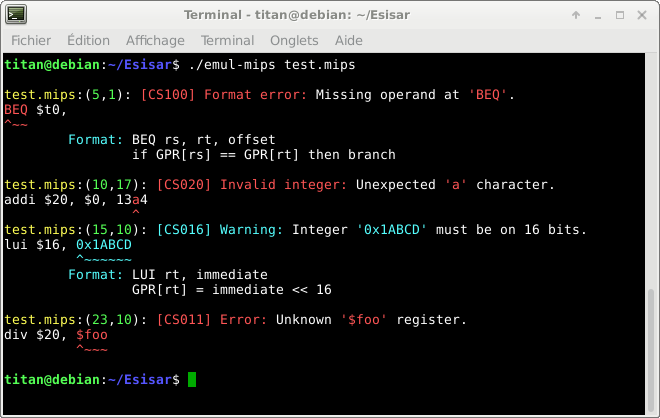
\includegraphics[width=\textwidth]{MIPS-mpError-exemple.png}
    \end{center}
    \caption{\\Exemple d'erreurs gérées par l'émulateur.}
    \label{simulationBER}
\end{figure}


% ========================================================== %
%     COMPILATION
% ========================================================== %
\chapter{Compilation}

\paragraph{}
Cette partie transforme une ligne composée de mots en valeurs sémantique, pour ensuite en déduire si une instruction est présente et si elle est correctement écrite avec les bonnes opérandes.

% ========================================================== %
%     COMPILATION : mpString
% ========================================================== %
\section{mpString}

\paragraph{}
Ce petit module définit quelques fonctions uselles sur les caracèteres et chaînes de caractères (Comme une fonction {\ttfamily mpStrCiCmp} pour comparer deux chaînes sans tenir compte de la casse, ou {\ttfamily mpGetFilename} qui retourne le nom du fichier pour un chemin donné). Mais aussi principalement une fonction {\ttfamily mpGetLine} qui retourne dans une {\ttfamily mpLine} la ligne courante d'un fichier sans tenir compte des commentaires.

%\vspace{5mm}
\begin{lstlisting}[
    style=CStyle,
    numbers=none,
    title={\ttfamily mpString.h}
]
bool
mpGetLine(
    FILE*    file,
    mpLine*  line,
    mpError* error
);
\end{lstlisting}

\paragraph{}
Cette fonction peut aussi retourner une erreur. En l'occurence la seule erreur possible ici est {\ttfamily mpErrorLINE\_OVERFLOW} quand la ligne courante du fichier est plus grande que le buffer de la ligne passée en paramètre. Pour pallier (entres autres) ce problème, une liste dynamique a été developpée fonctionnant de la même manière qu'un {\ttfamily std::vector} en {\ttfamily C++} et permettrait d'ajouter bien plus de caractères qu'actuellement. Cela est dû au fait que {\ttfamily mpLine} est une structure contenant un tableau fini de caractères de dimiension {\ttfamily mpLINE\_MAX} accompagné un entier non signé pour la taille :

%\vspace{5mm}
\begin{lstlisting}[
    style=CStyle,
    numbers=none,
    title={\ttfamily mpType.h}
]
#define mpLINE_MAX 81u

typedef struct
{
    mpChar text[mpLINE_MAX];
    size_t length;
}
mpLine;
\end{lstlisting}

\paragraph{}
La liste dynamique développée est disponible dans le code source et fonctionne aussi avec un type {\ttfamily template} comme en {\ttfamily C++}. Malheuresement le temps n'aura pas permis une implémentation pour {\ttfamily mpLine}.

Toutefois, la fonction {\ttfamily mpGetLine} possède un (autre) petit défaut : si le fichier a été engistré sous Windows les retours à la ligne seront codés avec les caractères "{\ttfamily \textbackslash r\textbackslash n}" et la fonction prendra ces deux caratères comme \textbf{deux} retours à la ligne (au lieu d'un). Le problème est juste visuel car si une erreur occure sur une ligne l'affichage du numéro sur la console ne correspond pas.


% Défaut pas géré  de Windows donc si erreur pas cool

% ========================================================== %
%     COMPILATION : mpToken
% ========================================================== %
\section{mpToken}
\label{section_mpToken}

\paragraph{}
Le module {\ttfamily mpToken} est important car il permet d'associer aux mots d'une ligne une étiquette et une valeur (respectivement {\ttfamily mpTag} et {\ttfamily mpValue}) dans un jeton ({\ttfamily mpToken}) :

%\vspace{5mm}
\noindent
\begin{minipage}[t]{.3\textwidth}
\begin{lstlisting}[
    style=CStyle,
    numbers=none,
    title={\ttfamily mpType.h}
]
typedef enum
{
    mpTagEND  = -1,
    mpTagNONE =  0,

    mpTagLEFT_BRACKET,
    mpTagRIGHT_BRACKET,
    mpTagCOMMA,
    mpTagCOLON,

    mpTagINSTRUCTION,
    mpTagREGISTER,
    mpTagINTEGER,
    mpTagLABEL
}
mpTag;
\end{lstlisting}
\end{minipage}\hfill
%
\begin{minipage}[t]{.3\textwidth}
\begin{lstlisting}[
    style=CStyle,
    numbers=none,
    title={\ttfamily mpType.h}
]
typedef union
{
    char  character;
    int   integer;
    void* pointer;
}
mpValue;
\end{lstlisting}
\end{minipage}\hfill
%
\begin{minipage}[t]{.3\textwidth}
\begin{lstlisting}[
    style=CStyle,
    numbers=none,
    title={\ttfamily mpType.h}
]
typedef struct
{
    mpTag   tag;
    mpValue value;
    mpChar* word;
}
mpToken;
\end{lstlisting}
\end{minipage}

\paragraph{}
{\ttfamily mpTag} est une énumération des différents types possibles, par exemple une paranthèse, un nombre ou bien encore un registre. {\ttfamily mpValue} est la valeur associée (si elle existe) au {\ttfamily mpTag}. Le dernier membre {\ttfamily word} de {\ttfamily mpToken} est juste un pointeur sur le début du mot à la ligne {\ttfamily mpLine} correspondant, mais ne modifie pas cette dernière pour ajouter un caractère de fin '{\ttfamily \textbackslash 0}'.

\paragraph{}
Pour extraire un {\ttfamily mpToken} d'une {\ttfamily mpLine} on appelle la fonction {\ttfamily mpFetchToken} qui retourne {\ttfamily true} tant qu'il a des mots à trouver dans la ligne. Chaque token est placé dans une liste et cette liste sera interprétée par le {\ttfamily mpTranspiler} de la partie \ref{section_mpTranspiler} page \pageref{section_mpTranspiler}.

%\vspace{5mm}
\noindent
\begin{minipage}[t]{.45\textwidth}
\begin{lstlisting}[
    style=CStyle,
    numbers=none,
    title={\ttfamily mpToken.h}
]
bool
mpFetchToken(
    mpFetch* fetch,
    mpError* error
);
\end{lstlisting}
\end{minipage}\hfill
%
\begin{minipage}[t]{.45\textwidth}
\begin{lstlisting}[
    style=CStyle,
    numbers=none,
    title={\ttfamily mpToken.h}
]
void
mpFetchInit(
    mpFetch* fetch,
    mpLine*  line
);
\end{lstlisting}
\end{minipage}

\paragraph{}
{\ttfamily mpFetch} est une structure permettant de garder le contexte du parcours d'une ligne tout en retournant un {\ttfamily mpToken} à chaque fois qu'un mot est décodé, il faut impérativement initialiser cette structure avec {\ttfamily mpFetchInit} avant de l'utiliser.

\begin{lstlisting}[
    style=CStyle,
    numbers=none,
    title=Exemple d'utilisation :
]
mpFetchInit(&fetch, &line);

while (mpFetchToken(&fetch, &error))
{
    if (error.success)
    {
        (*@\color{mGreen}{\ttfamily // Faire quelque chose avec fetch.token}@*)
    }
}
\end{lstlisting}

    % ========================================================== %
    %     COMPILATION : mpToken : Ponctuation
    % ========================================================== %
    \subsection{La ponctuation}
    \paragraph{}
    Comme on peut le voir dans {\ttfamily mpTag}, la ponctuation de l'émulateur {\ttfamily MIPS} comprend les parenthèses ouvrantes '{\ttfamily (}' et fermantes '{\ttfamily )}', ainsi que les virgules '{\ttfamily ,}' et les deux-points '{\ttfamily :}' (Pour les labels, bien qu'ils n'aient pas été implémentés). Si une autre ponctuation est trouvée alors une erreur sera remontée à l'utilisateur et l'émulation du programme demandée n'aura pas lieu.

    Aucune valeur n'est placée dans le champ {\ttfamily mpValue} du {\ttfamily mpToken} car le {\ttfamily mpTag} se suffit à lui-même. Ci-dessous un exemple d'erreur affichée à l'utilisateur :

    \begin{center}
        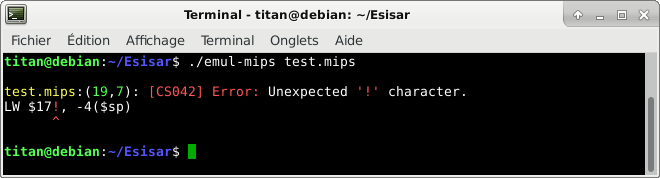
\includegraphics[width=\textwidth]{MIPS-mpToken-ponctuation.png}
    \end{center}

    % ========================================================== %
    %     COMPILATION : mpToken : nombres
    % ========================================================== %
    \subsection{Les nombres}

    \paragraph{}
    Les nombres peuvent être écrit en base binaire, octal, décimal et hexadécimal avec en option le caractère '{\ttfamily -}' ou '{\ttfamily +}' pour indiquer le signe.
    \begin{itemize}
        \setlength\itemsep{1em}

        \item \textbf{Base 2 :}

        Commence par le suffixe "{\ttfamily 0b}" suivit des chiffres '{\ttfamily 0}' et '{\ttfamily 1}'. Le type d'erreur associé est {\ttfamily mpErrorBINARY\_FORMAT}.

        \item \textbf{Base 8 :}

        Commence obligatoirement par un zéro '{\ttfamily 0}' (comme en {\ttfamily C}) suivit des chiffres entre '{\ttfamily 0}' et '{\ttfamily 7}'. Une erreur de type {\ttfamily mpErrorOCTAL\_FORMAT} est remontée dans le cas contraire.

        \item \textbf{Base 10 :}

        Contient les chiffres entre '{\ttfamily 0}' et '{\ttfamily 9}' mais ne doit pas commencer par un '{\ttfamily 0}' sinon il sera decodé comme un nombre en base octal. Le type d'erreur associé est {\ttfamily mpErrorINTEGER\_FORMAT}.

        \item \textbf{Base 16 :}

        Commence par le suffixe "{\ttfamily 0x}" avec les chiffres entre '{\ttfamily 0}' et '{\ttfamily 9}' et les caractère entre '{\ttfamily A}' et '{\ttfamily F}', le décodage est insensible à la casse. Le type d'erreur associé est {\ttfamily mpErrorHEX\_FORMAT}.
    \end{itemize}

    \paragraph{} À ce stade de la compilation aucune vérification n'est faite sur le nombre maximum de bits autorisés pour réprésenter un nombre. Si aucune erreur de syntaxe n'est détectée on définit le {\ttfamily mpTag} comme un {\ttfamily mpTagINTEGER}, et on stocke la valeur décodée dans le membre {\ttfamily integer} de {\ttfamily mpValue}.

\begin{lstlisting}[
    style=CStyle,
    numbers=none,
    title=Exemple :
]
token.tag           = mpTagINTEGER;
token.value.integer = value; (*@\color{mGreen}{\ttfamily // Valeur décodée auparavant}@*)
\end{lstlisting}


    % ========================================================== %
    %     COMPILATION : mpToken : registres
    % ========================================================== %
    \subsection{Les registres}
    \paragraph{}
    Les registres commencent tous par un dollar '{\ttfamily \$}' et sont suivis soit d'un nombre en {\ttfamily 0} et {\ttfamily 31}, soit de leur mnémonique associée (par exemple {\ttfamily a0}, {\ttfamily a1}, {\ttfamily sp}, {\ttfamily ra}, etc) sans tenir compte de la casse. Si le registre indiqué n'est pas valide une erreur sera affichée à l'utilisateur et l'émulation du programme ne se lancera pas. Exemple d'erreur :

    \begin{center}
        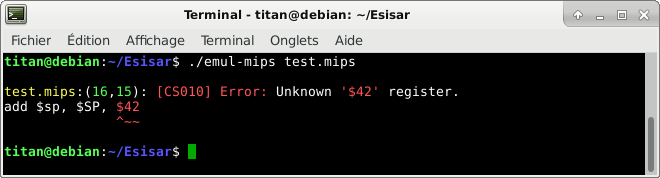
\includegraphics[width=\textwidth]{MIPS-mpToken-registre.png}
    \end{center}

    \paragraph{}
    De la même façon que pour les nombres on définit les valeurs du {\ttfamily mpToken} comme suit :

\begin{lstlisting}[
    style=CStyle,
    numbers=none,
    title=Exemple :
]
token.tag           = mpTagREGISTER;
token.value.integer = theRegister; (*@\color{mGreen}{\ttfamily // numéro du registre décodée auparavant}@*)
\end{lstlisting}


    % ========================================================== %
    %     COMPILATION : mpToken : instructions
    % ========================================================== %
    \subsection{Les instructions (mnémonique)}

    \paragraph{}
    Les instructions valides sont strockées dans une liste qui sera expliquée dans la partie \ref {section_mpTranspiler}. Les instructions sont triées par ordre alphabétique de leur mnémonique et une fonction {\ttfamily mpGetInstruction} regarde si un mot donné est un mnémonique valide avec une recherche dichotomique (sans tenir compte de la casse).

    \paragraph{}
    À la différence des autres types, on place dans la valeur {\ttfamily mpValue} du {\ttfamily mpToken} un pointeur vers un structure {\ttfamily mpInstruction} qui sera expliqué dans la partie \ref{section_mpInstruction}, ce pointeur est retourné par la fonction {\ttfamily mpGetInstruction} en cas de succès. Si le pointeur est {\ttfamily NULL} et que le mot ne correspond à aucun autres types, et qu'il est composé uniquement de caractères alpha-numériques, alors il est considéré comme un label.

\begin{lstlisting}[
    style=CStyle,
    numbers=none,
    title=Exemple :
]
token.tag           = mpTagINSTRUCTION;
token.value.pointer = (void*) instruction;
\end{lstlisting}

    % ========================================================== %
    %     COMPILATION : mpToken : Autres
    % ========================================================== %
    \subsection{Autres}
    \paragraph{} Si un mot commence par un point '{\ttfamily .}' il est alors considéré comme une directive, mais une erreur sera directement remontée à l'utilisateur car elles ne sont pas supportées. De même pour les labels :

    \begin{center}
        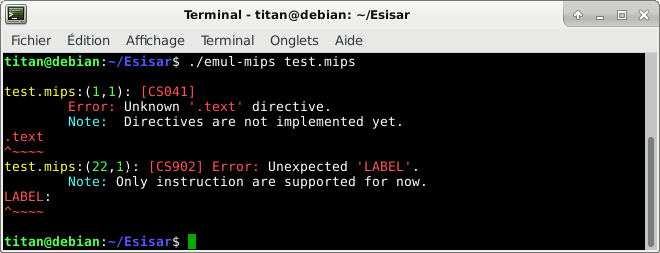
\includegraphics[width=\textwidth]{MIPS-mpToken-directive-label.png}
    \end{center}

% ========================================================== %
%     COMPILATION : mpInstruction
% ========================================================== %
\section{mpInstruction}
\label{section_mpInstruction}

\paragraph{}
Ce module s'occupe de convertir la liste de {\ttfamily mpToken} créée dans la partie \ref{section_mpToken} en une instruction de 32 bits. Tout d'abord on définit deux types, une structure {\ttfamily mpInstruction} qui définit une instruction avec un {\ttfamily opcode}, une mnémonique, une description accompagnée d'un format (ces deux derniers servent uniquement à l'affichage) et une fonction {\ttfamily mpToMemory} qui va écrire dans l'instruction dans la mémoire.

%\vspace{5mm}
\noindent
\begin{minipage}[t]{.45\textwidth}
\begin{lstlisting}[
    style=CStyle,
    numbers=none,
    title={\ttfamily mpInstruction.h}
]
typedef void
(*mpToMemory)(
    mpInstruction*    inst,
    mpVector_mpToken* tokens,
    mpMemory*         memory,
    mpError*          error
);
\end{lstlisting}
\end{minipage}\hfill
%
\begin{minipage}[t]{.45\textwidth}
\begin{lstlisting}[
    style=CStyle,
    numbers=none,
    title={\ttfamily mpInstruction.h}
]
typedef struct
{
    int        opcode;
    mpCString  mnemonic;
    mpToMemory ToMemory;

    mpCString format;
    mpCString description;
}
mpInstruction;
\end{lstlisting}
\end{minipage}

\paragraph{}
Ensuite une liste complète des 26 instructions supportées est définie :


\begin{lstlisting}[
    style=CStyle,
    numbers=none,
    title={\ttfamily mpInstruction.c}
]
static
mpInstruction const s_instruction[mpINSTRUCTION_MAX] =
{
    {
        mpADD_OPCODE,
        "ADD",
        mpRtype_ORRR,
        "rd, rs, rt",
        "GPR[rd] = GPR[rs] + GPR[rt]"
    },
    {
        mpADDI_OPCODE,
        "ADDI",
        mpItype_ORRI,
        "rt, rs, immediate",
        "GPR[rt] = GPR[rs] + immediate"
    },
    (*@\dots@*)
};
\end{lstlisting}

\paragraph{}
Avant d'écrire dans la mémoire, les fonctions  {\ttfamily mpToMemory} vérifient si les étiquettes {\ttfamily mpTag} de la liste de {\ttfamily mpToken} correspondent bien à une syntaxe valide. Prenons l'exemple avec de l'instruction {\ttfamily ADD} décrite ci-dessus, on observe que la structure contient une fonction {\ttfamily mpRtype\_ORRR} :

%\vspace{5mm}
\noindent
\begin{minipage}[t]{.45\textwidth}
\begin{lstlisting}[
    style=CStyle,
    numbers=none,
    title={\ttfamily mpInstruction.c}
]
static
mpTag const s_ORRR[] =
{
    mpTagINSTRUCTION,
    mpTagREGISTER,
    mpTagCOMMA,
    mpTagREGISTER,
    mpTagCOMMA,
    mpTagREGISTER,
    mpTagEND
};
\end{lstlisting}
\end{minipage}\hfill
%
\begin{minipage}[t]{.45\textwidth}
\begin{lstlisting}[
    style=CStyle,
    numbers=none,
    title={\ttfamily mpInstruction.c}
]
void
mpRtype_ORRR (
    mpInstruction*    inst,
    mpVector_mpToken* tokens,
    mpMemory*         memory,
    mpError*          error
) {
    mpMatchTag(
        tokens, s_ORRR, error);

    if (error->success)
    {
        mpWriteRtype(memory, (*@\dots@*));
    }
}
\end{lstlisting}
\end{minipage}

\paragraph{}
Dans un premier temps cette fonction va comparer les {\ttfamily mpTag} de la liste de  {\ttfamily mpToken} avec un tableau de {\ttfamily mpTag} prédéfini. Si cette comparaison est un succès au {\ttfamily mpTag} près sans un en trop ou en moins, alors une fonction s'occupe de récupérer les valeurs {\ttfamily mpValue} pour écrire correctement l'instruction sur 32 bits. Cette dernière fonction {\ttfamily mpWriteInstruction} sera expliquée dans le chapitre \ref{chaptire_mem_reg} page \pageref{chaptire_mem_reg} sur la mémoire et les registres.

\begin{lstlisting}[
    style=CStyle,
    numbers=none,
    title={\ttfamily mpInstruction.c}
]
static
void
mpWriteRtype (
    mpMemory* memory,
    int op, int sa,
    int rd, int rs, int rt
) {
    uint32_t hex = 0;

    hex |= (uint32_t)((op & 0x3F));
    hex |= (uint32_t)((sa & 0x1F) << 6);
    hex |= (uint32_t)((rd & 0x1F) << 11);
    hex |= (uint32_t)((rt & 0x1F) << 16);
    hex |= (uint32_t)((rs & 0x1F) << 21);

    mpWriteInstruction(memory, hex);
}
\end{lstlisting}

\paragraph{}
Quelques exemples d'erreurs :

\begin{center}
    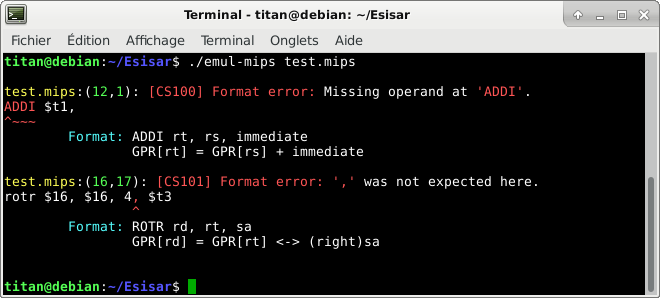
\includegraphics[width=\textwidth]{MIPS-mpInstruction.png}
\end{center}

\paragraph{}
Cette méthode est répétée autant de fois pour chacune des 26 instructions avec des fonctions qui leur sont adaptées. Cette archictecture permet une grande maintenabilité avec beaucoup de factorisations de code mais n'est cependant pas tant maléable que ça.

% ========================================================== %
%     COMPILATION : mpTranspiler
% ========================================================== %
\section{mpTranspiler}
\label{section_mpTranspiler}

\paragraph{}
Le {\ttfamily mpTranspiler} fait la jonction entre tous les modules de ce chapitre. La fonction {\ttfamily mpTranspiler} prend en paramètres le nom du fichier à émuler et une mémoire où écrire les instructions :

\begin{lstlisting}[
    style=CStyle,
    numbers=none,
    title={\ttfamily mpTranspiler.h}
]
void
mpTranspiler(
    mpCString filename,
    mpMemory* memory,
    mpError*  error
);
\end{lstlisting}

\paragraph{}
Des sous-routines existent, une pour ouvrir le fichier et traiter les erreurs, une autres pour récupèrer proprement une ligne dans le fichier, et une dernière pour récupérer une liste de {\ttfamily mpToken} et l'envoyer à la mémoire. Cette dernière fonction présentée ci-dessous est importante car elle est réutilisée pour le mode intéractif :

\begin{lstlisting}[
    style=CStyle,
    numbers=none,
    title={\ttfamily mpTranspiler.h}
]
void
mpTranspiler_FetchToken(
    mpLine*   line,
    mpMemory* memory,
    mpError*  error
);
\end{lstlisting}

\paragraph{}
Ces fonction peuvent aussi faire remonter des erreurs, comme annoncer que le fichier envoyé n'existe pas ou encore que le fichier est vide :

\begin{center}
    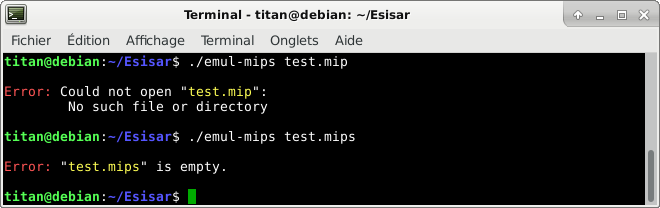
\includegraphics[width=\textwidth]{MIPS-mpTranspiler.png}
\end{center}

% ========================================================== %
%     MEMOIRE ET REGISTRE
% ========================================================== %
\chapter{Mémoire et Registres}
\label{chaptire_mem_reg}

\paragraph{} Bla bla

% ========================================================== %
%      MEMOIRE ET REGISTRE : mpRegister
% ========================================================== %
\section{mpRegister}

\paragraph{}
La gestion de registres est très simple, il s'agit tout simplement d'un tableau de {\ttfamily 32} registre {\ttfamily +} {\ttfamily 4} registres spéciaux :


\begin{lstlisting}[
    style=CStyle,
    numbers=none,
    title={\ttfamily mpRegister.h}
]
#define mpUSUAL_REGISTER   32u
#define mpSPECIAL_REGISTER 4u

typedef union
{
    uint32_t    GPR[mpUSUAL_REGISTER + mpSPECIAL_REGISTER];
    mpRegister_ all;
}
mpRegister;
\end{lstlisting}

\paragraph{}
Ce tableau est placé dans un {\ttfamily union} avec une structure composée de tous les registres et leur mnémonique. De cette façon, on peut accèder à un registre par deux moyens, soit utiliant le tableau {\ttfamily GPR}, soit par la structure {\ttfamily all}, cette fonctionnalité a pour seul but d'apporter une meilleur lisibilité du code quand on souhaite accèder à un registre en particulier, sinon on utilisera le tableau.

\begin{lstlisting}[
    style=CStyle,
    numbers=none,
    title={\ttfamily mpRegister.h}
]
typedef struct
{
    (*@\color{mGreen}{\ttfamily /* Registres */}@*)
    uint32_t zero;
    uint32_t at;
    uint32_t v0, v1;
    uint32_t a0, a1, a2, a3;
    uint32_t t0, t1, t2, t3, t4, t5, t6, t7;
    uint32_t s0, s1, s2, s3, s4, s5, s6, s7;
    uint32_t t8, t9;
    uint32_t k0, k1;
    uint32_t gp, sp, fp, ra;
    (*@\color{mGreen}{\ttfamily /* Registres spéciaux */}@*)
    uint32_t pc, ir;
    uint32_t hi, lo;
}
mpRegister_;
\end{lstlisting}

\paragraph{}
On accompagne les registres d'une fonction pour les afficher proprement à l'utilisateur :

\begin{center}
    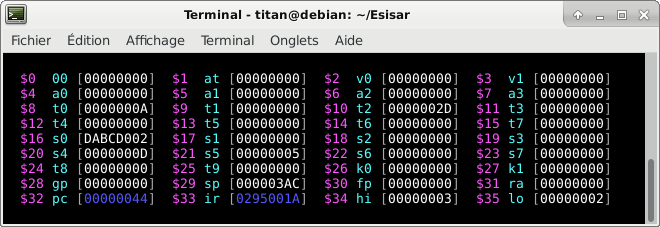
\includegraphics[width=\textwidth]{MIPS-mpRegister.png}
\end{center}

% ========================================================== %
%      MEMOIRE ET REGISTRE : mpMemory
% ========================================================== %
\section{mpMemory}

\paragraph{}
La mémoire se compose simplement d'un tableau d'octets avec un invertalle [ {\ttfamily minAddress}, {\ttfamily maxAddress} ] pour autoriser la lecture et l'écriture, le reste étant en lecture seule. Le choix d'avoir un tableau d'octet (8 bits) a été préféré par rapport à un tableau d'entier (32 bits) pour coller au plus à un processeur {\ttfamily MIPS}. {\ttfamily minAddress} est intialisée à {\ttfamily 0} avant la partie compilation puis s'incrémente de {\ttfamily 4} à chaque ajoute d'instruction,

\begin{lstlisting}[
    style=CStyle,
    numbers=none,
    title={\ttfamily mpMemory.h}
]
#define mpMEMORY_MAX 1024

typedef struct
{
    uint8_t  octet[mpMEMORY_MAX];
    uint32_t minAddress;
    uint32_t maxAddress;
}
mpMemory;
\end{lstlisting}

\paragraph{}
Sont fournis avec la mémoire deux fonctions, une pour la lecture et l'autre pour l'écriture, et dans lesquelles est testé la valeur {\ttfamily address} avec les bornes de la mémoire. Le cas échant une erreur est remontée et l'émuation est stoppée. La fonction {\ttfamily mpWriteInstruction} correspondant à un {\ttfamily mpStoreWord} à l'adresse {\ttfamily minAddress} tout en l'incrémentant de {\ttfamily 4} après.

%\vspace{5mm}
\noindent
\begin{minipage}[t]{.45\textwidth}
\begin{lstlisting}[
    style=CStyle,
    numbers=none,
    title={\ttfamily mpMemory.h}
]
uint32_t
mpLoadWord (
    mpMemory* memory,
    uint32_t  address,
    mpError*  error
);
\end{lstlisting}
\end{minipage}\hfill
%
\begin{minipage}[t]{.45\textwidth}
\begin{lstlisting}[
    style=CStyle,
    numbers=none,
    title={\ttfamily mpMemory.h}
]
void
mpStoreWord (
    mpMemory* memory,
    uint32_t  address,
    uint32_t  value,
    mpError*  error
);
mpInstruction;
\end{lstlisting}
\end{minipage}

\paragraph{}
Il existe une constante {\ttfamily mpBIG\_ENDIAN} qui permet d'indiquer dans quelle ordre on souhaite écrire nos données en mémoire. Si cette constante est à {\ttfamily 1} alors on écrit les données en \textit{big endian} sinon en \textit{little endian}.

\begin{lstlisting}[
    style=CStyle,
    numbers=none,
    title={\ttfamily mpMemory.h}
]
#define mpBIG_ENDIAN 1
\end{lstlisting}

\paragraph{}
La mémoire est aussi accompagnée d'un fonction pour l'afficher à utilisateur. Cette fonction prend en paramètre une borne d'adresse sur laquelle centrer le contenue. Ci-dessous, le premier bloc est centré sur le {\ttfamily PC} et le deuxième sur le {\ttfamily SP}.

\begin{center}
    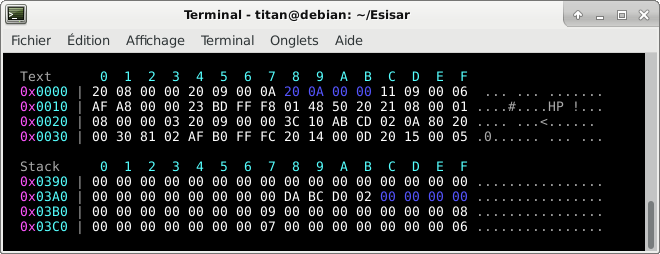
\includegraphics[width=\textwidth]{MIPS-mpMemory.png}
\end{center}

% ========================================================== %
%     EMULATEUR
% ========================================================== %
\chapter{Émulateur}

% ========================================================== %
%     EMULATEUR : mpEmulator
% ========================================================== %
\section{mpEmulator}

    \paragraph{}
    dzadza dza

    \subsection{Exécution d'une instruction}

    \paragraph{}
    \dots
    %Pour exécuter une instruction il existe trois fonction : {\ttfamily mpRtype}, {\ttfamily mpItype} et {\ttfamily mpJtype}. Chaque fonction prend en paramètre une instruction codée sur 32 bits et la décode en fonction de son type.

    %\paragraph{}
    %Une fonction {\ttfamily mpEmulator\_Step} se charge de récupérer l'instruction courante à partir du {\ttfamily PC}, puis de la placer dans le registre {\ttfamily IR} pour ensuite appeler l'une des trois fonction décrite plus haut.


    % ========================================================== %
    %     EMULATEUR : Mode simple
    % ========================================================== %
    \subsection{Mode simple}

    \paragraph{}
    Ce mode permet d'émuler un programme écrit en {\ttfamily MIPS} et d'avoir directement le résultat à afficher sur la console.

\begin{center}
    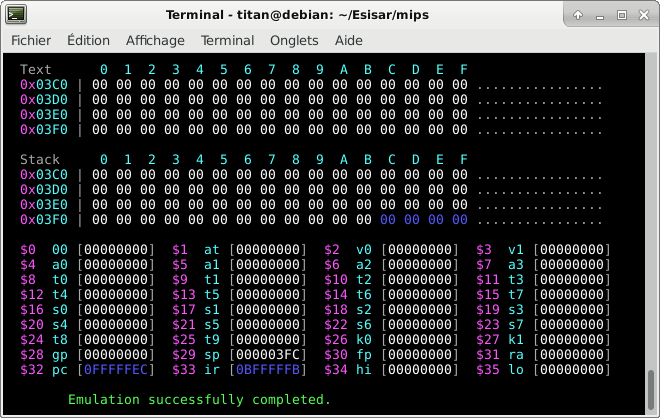
\includegraphics[width=\textwidth]{MIPS-mpEmulator-ModeSimple.png}
\end{center}


    % ========================================================== %
    %     EMULATEUR : Mode pas à pas
    % ========================================================== %
    \subsection{Mode pas à pas}

    \paragraph{}
    Ce mode reprend le mode simple mais avec la possibilité d'exécuter les instructions pas à pas, c'est-à-dire en appuyant sur la touche {\ttfamily ENTRÉE} pour passer à une instruction suivante.

\begin{center}
    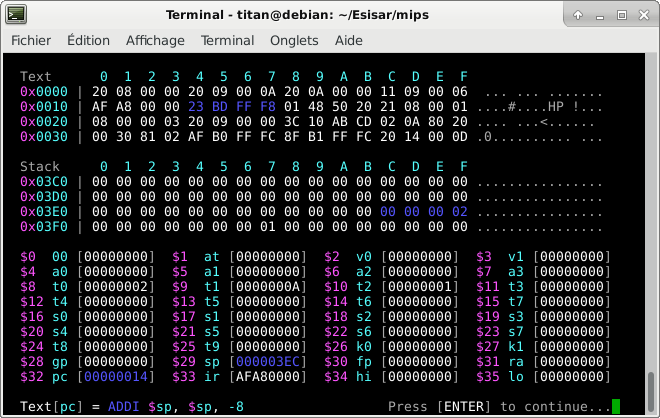
\includegraphics[width=\textwidth]{MIPS-mpEmulator-ModePasPas.png}
\end{center}

    % ========================================================== %
    %     EMULATEUR : intéractif
    % ========================================================== %
    \subsection{Mode intéractif}

    \paragraph{}
    Le mode intéractif laisse la possibilité à l'utilisateur d'entrer ses instructions à souhait.

\begin{center}
    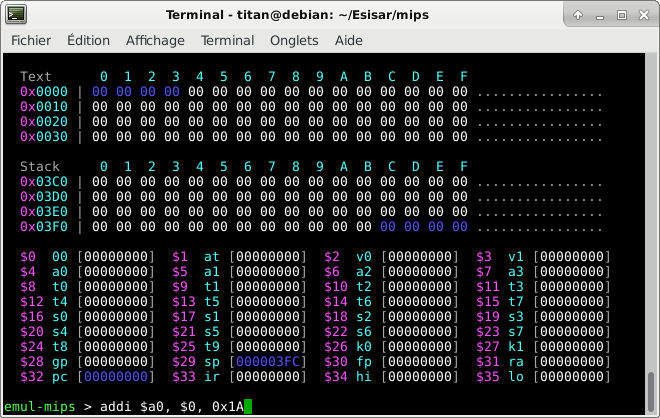
\includegraphics[width=\textwidth]{MIPS-mpEmulator-ModeInteractif.png}
\end{center}

% ========================================================== %
%     EMULATEUR : main
% ========================================================== %
\section{main}

\paragraph{}
\dots

% ========================================================== %
%     CONCLUSION
% ========================================================== %
\chapter{Conclusion}

\paragraph{}
Ce projet était très intéressant à réaliser. Avec plus de temps il aurait été possible de faire un projet bien plus complet, c'est pourquoi je garde mes idées dans un coin pour, pourquoi pas, un jour retravailler dessus.

\end{document}